%%%%%%%%%%%%%%%%%%%%%%%%%%%%%%%%%%%%%%%%%
% Short Sectioned Assignment
% LaTeX Template
% Version 1.0 (5/5/12)
%
% This template has been downloaded from:
% http://www.LaTeXTemplates.com
%
% Original author:
% Frits Wenneker (http://www.howtotex.com)
%
% License:
% CC BY-NC-SA 3.0 (http://creativecommons.org/licenses/by-nc-sa/3.0/)
%
%%%%%%%%%%%%%%%%%%%%%%%%%%%%%%%%%%%%%%%%%

%----------------------------------------------------------------------------------------
%	PACKAGES AND OTHER DOCUMENT CONFIGURATIONS
%----------------------------------------------------------------------------------------

\documentclass[paper=a4, fontsize=11pt]{scrartcl} % A4 paper and 11pt font size
\usepackage{listings}
\usepackage{graphicx}
\usepackage{float}
\usepackage[T1]{fontenc} % Use 8-bit encoding that has 256 glyphs
\usepackage{fourier} % Use the Adobe Utopia font for the document - comment this line to return to the LaTeX default
\usepackage[english]{babel} % English language/hyphenation
\usepackage{amsmath,amsfonts,amsthm} % Math packages
\usepackage{fancyvrb}
\usepackage{lipsum} % Used for inserting dummy 'Lorem ipsum' text into the template
\usepackage[utf8x]{inputenc}

\usepackage{sectsty} % Allows customizing section commands
\allsectionsfont{\centering \normalfont\scshape} % Make all sections centered, the default font and small caps

\usepackage{fancyhdr} % Custom headers and footers
\pagestyle{fancyplain} % Makes all pages in the document conform to the custom headers and footers
\fancyhead{} % No page header - if you want one, create it in the same way as the footers below
\fancyfoot[L]{} % Empty left footer
\fancyfoot[C]{} % Empty center footer
\fancyfoot[R]{\thepage} % Page numbering for right footer
\renewcommand{\headrulewidth}{0pt} % Remove header underlines
\renewcommand{\footrulewidth}{0pt} % Remove footer underlines
\setlength{\headheight}{0pt} % Customize the height of the header

\numberwithin{equation}{section} % Number equations within sections (i.e. 1.1, 1.2, 2.1, 2.2 instead of 1, 2, 3, 4)
\numberwithin{figure}{section} % Number figures within sections (i.e. 1.1, 1.2, 2.1, 2.2 instead of 1, 2, 3, 4)
\numberwithin{table}{section} % Number tables within sections (i.e. 1.1, 1.2, 2.1, 2.2 instead of 1, 2, 3, 4)

\setlength\parindent{0pt} % Removes all indentation from paragraphs - comment this line for an assignment with lots of text

%----------------------------------------------------------------------------------------
%	TITLE SECTION
%----------------------------------------------------------------------------------------

\newcommand{\horrule}[1]{\rule{\linewidth}{#1}} % Create horizontal rule command with 1 argument of height

\title{	
\normalfont \normalsize 
\textsc{alma mater studiorum - università di bologna} \\ [25pt] % Your university, school and/or department name(s)
\horrule{0.5pt} \\[0.4cm] % Thin top horizontal rule
\huge Documentazione smallNorbCreator v.0.3 \\ % The assignment title
\horrule{0.5pt} \\[0.5cm] % Thick bottom horizontal rule
}

\author{Vincenzo Lomonaco} % Your name

\date{\normalsize\today} % Today's date or a custom date

\begin{document}

\maketitle % Print the title

%----------------------------------------------------------------------------------------
%	PROBLEM 1
%----------------------------------------------------------------------------------------

\section{Introduzione}

Il progetto \emph{smallNorbCreator} ha come obiettivo la creazione di un meta-database di sequenze di immagini a partire dal database \emph{``small NORB v.1.0''} orginale.
Ad oggi è composto da 7 sorgenti java ed un jar eseguibile:

\begin{enumerate}
	\item NorbConverter.java
	\item NorbSampler.java
	\item NorbSamplerTrain.java
	\item NorbSamplerTest.java 
	\item NorbSeqExplorer.java
	\item NorbKNN.java 
	\item NorbCreator.java
	\item norbCreator.jar
\end{enumerate}

\section{NorbConverter.java}
\emph{NorbConverter.java} si occupa della conversione delle immagini originali dal formato matlab a quello bitmap eseguendo eventualmente un sottocampionamento delle immagini e dividendole per classi in sottocartelle differenti.

\section{NorbSampler.java}
\emph{NorbSampler.java} è una classe astratta che viene ereditata dalle sottoclassi \emph{NorbSamplerTrain.java} e \emph{NorbSamplerTest.java}. Essa si occupa di implementare le funzionalità di base offerte da un generatore di sequenze di base, a prescindere esse siano di train o di test.

\section{NorbSamplerTrain.java}
\emph{NorbSamplerTrain.java} si occupa del sampling del training set.
Innanzitutto si parte dal presupposto che training set e test set siano riuniti in un unica cartella contenente le 5 sottocartelle rispettive a ciascuna classe 0,1,2,3,4.
Per ogni oggetto presente in queste directory una o più sequenze di immagini possono essere create. Le sequenze hanno lunghezza arbitraria e sono caratterizzate da una singola variazione unitaria di frame in frame in una sola delle dimensioni possibili tra elevazione, azimuth e illuminazione. Ognuna di queste possibili variazioni ha una certa probabilità. Ad esse si aggiunge quella del cambiamento di direzione delle variazioni. Alla fine tutti i parametri di cui sopra e le sequenze di immagini vengono scritte all'interno di un'unico file di testo.

\subsection{Il formato del file di output}
il formato per il file di output del training set che viene creato una volta lanciato il programma è un file di testo semplice la cui intestazione contiene le seguenti informazioni:

\begin{itemize}
\item \emph{Config Type}: Tipo del file di configurazione, in questo caso ``Train''.
\item \emph{nClass}: numero di classi da considerare (vengono prese in considerazione le classi da indice 0 a n-1).
\item \emph{nObjxClass}: numero di oggetti da considerare per classe (vengono prese in considerazione gli oggetti da indice 0 a n-1).
\item \emph{nSeqxObj}: numero di sequenze di immagini da creare per ciascun oggetto.
\item \emph{elevationProb}: Probabilità che la variazione tra un frame e l'altro riguardi l'elevazione (un incremento o decremento della dell'elevazione ha uuguale probabilità).
\item \emph{azimuthProb}: Probabilità che la variazione tra un frame e l'altro riguardi l'azimuth (un incremento o decremento della dell'azimuth ha uguale probabilità).
\item \emph{lightingProb}: Probabilità che la variazione tra un frame e l'altro riguardi la luminosità (un incremento o decremento della dell'illuminazione ha uguale probabilità).
\item \emph{flipProb}: Probabilità di cambiare direzione di variazione.
\item \emph{seqLen}: Lunghezza di ciascuna sequenza.
\item \emph{seed}: Seme per il generatore di numeri pseudo-casuali.
\end{itemize}

In Fig. \ref{img:trainheader} è possibile osservare un esempio di intestazione del file di configurazione generato a seguito dell'esecuzione dello script \emph{NorbSamplerTrain.java}.
In seguito, precedute da una linea vuota e da un'intestazione specifica della sequenza vi sono tutte le immagini costituenti la stessa identificate dal loro nome.
L'intestazione contiene gli indici rispettivi alla classe, all' oggetto ed alla sequenza, come è possibile osservare in Fig.
 \ref{img:seqheader}.

\begin{figure}[H]
\label{img:trainheader}
\centering
\begin{BVerbatim}
Config Type: Train
-------------------------
nClass: 2
nObjxClass: 10
nSeqxObj: 1
ElevationProb: 0.3
AzimuthProb: 0.3
LightingProb: 0.2
FlipProb: 0.2
seqLen: 20
seed: 1234
-------------------------
\end{BVerbatim}
\caption{Un esempio di intestazione del file di configurazione per il training set.}
\end{figure}

\begin{figure}[H]
\label{img:seqheader}
\centering
\begin{BVerbatim}
---------------
Class:    0
Object:   0
Sequence: 0
---------------
00_02_10_05.bmp
00_03_10_05.bmp
00_03_12_05.bmp
00_04_12_05.bmp
00_05_12_05.bmp
00_06_12_05.bmp
00_07_12_05.bmp
...
\end{BVerbatim}
\caption{Un esempio di sequenza con relativa intestazione.}
\end{figure}

\section{NorbSamplerTest.java}
\emph{NorbSamplerTest.java} si occupa del sampling del test set. Leggendo i dati presenti nel file di configurazione del training set, esso genera per ogni oggetto una sequenza di immagini della stessa lunghezza di quelle create nel training set ma in cui ogni frame ha una distanza minima paramentrica da quelle utilizzate nel training set per lo stesso oggetto. In particolare la distanza tra due frame è calcolata come la somma delle variazioni su ciascuna dimensione. L'unico paramentro tarabile che differisce dal training set è dunque il numero di sequenze da creare per ciascun oggetto. Anche in questo caso alla fine tutti i parametri, le sequenze di immagini e la distanza media dal training set, vengono scritte all'interno di un'unico file di testo (vd. \emph{test\_conf.txt} in allegato). 

\subsection{Il formato del file di output}
Anche il formato per il file di output del test set che viene creato una volta lanciato il programma \emph{NorbSamplerTest.java} è un file di testo semplice la cui intestazione contiene le seguenti informazioni:

\begin{itemize}
\item \emph{Config Type}: Tipo del file di configurazione, in questo caso ``Test''.
\item \emph{nClass}: numero di classi da considerare (vengono prese in considerazione le classi da indice 0 a n-1).
\item \emph{nObjxClass}: numero di oggetti da considerare per classe (vengono prese in considerazione gli oggetti da indice 0 a n-1).
\item \emph{nSeqxObj}: Numero di sequenze da creare per ciascun oggetto.
\item \emph{elevationProb}: Probabilità che la variazione tra un frame e l'altro riguardi l'elevazione (un incremento o decremento della dell'elevazione ha uguale probabilità).
\item \emph{azimuthProb}: Probabilità che la variazione tra un frame e l'altro riguardi l'azimuth (un incremento o decremento della dell'azimuth ha uguale probabilità).
\item \emph{lightingProb}: Probabilità che la variazione tra un frame e l'altro riguardi la luminosità (un incremento o decremento della della luminosità ha uguale probabilità).
\item \emph{flipProb}: Probabilità di cambiare direzione di variazione.
\item \emph{seqLen}: Lunghezza di ciascuna sequenza.
\item \emph{seed}: Seme per il generatore di numeri pseudo-casuali.
\item \emph{min distance}: Minima distanza tra ciascun frame del training set e del test set rispetto a ciascun oggetto.
\end{itemize}

In Fig.\ref{img:testheader} è possibile osservare un esempio di intestazione del file di configurazione generato a seguito dell'esecuzione dello script \emph{NorbSamplerTest.java}.
In seguito, precedute da una linea vuota e da un'intestazione specifica della sequenza vi sono tutte le immagini costituenti la stessa, identificate dal loro nome.
Ogni sequenza ha un'intestazione contenente gli indici rispettivi alla classe, all' oggetto ed alla sequenza come è possibile osservare in Fig. \ref{img:seqheaderTest}. Dunque, riguardo il formato, non vi sono differenze rispetto alle sequenze generate nel training set.

\begin{figure}[H]
\label{img:testheader}
\centering
\begin{BVerbatim}
Config Type: Test
-------------------------
nClass: 2
nObjxClass: 10
nSeqxObj: 1
ElevationProb: 0.3
AzimuthProb: 0.3
LightingProb: 0.2
FlipProb: 0.2
seqLen: 20
seed: 1234
minDistance: 3
-------------------------
\end{BVerbatim}
\caption{Un esempio di intestazione del file di configurazione per il test set.}
\end{figure}

\begin{figure}[H]
\label{img:seqheaderTest}
\centering
\begin{BVerbatim}
---------------
Class:    0
Object:   0
Sequence: 0
---------------
00_00_16_03.bmp
00_00_18_03.bmp
00_01_18_03.bmp
00_01_18_02.bmp
00_02_18_02.bmp
00_03_18_02.bmp
00_02_18_02.bmp
...
\end{BVerbatim}
\caption{Un esempio di sequenza con relativa intestazione.}
\end{figure}

\section{NorbSeqExplorer.java}
\emph{NorbSeqExplorer.java} è un browser di immagini che si propone  di offrire un interfaccia agevole per la visualizzazione delle sequenze create mediante gli script \emph{NorbSamplerTrain.java} e \emph{NorbSamplerTest.java}. In Fig \ref{img:seqexplorer} si riporta un esempio di utilizzo. Mediante l'interfaccia è possibile specificare il file di configurazione da utilizzare (che sia di train o di test) e la directory principale nella quale sono contenute tutte le immagini separate per classe. Fatto ciò è possibile navigare le sequenze modificando i campi di input testuali e premendo invio oppure pigiando i bottoni laterali ``prev'' e ``next''. Si evidenzia che il codice in questione è ancora in uno stadio prematuro e non contiene adeguati controlli di sicurezza. Ad esempio, non offre ancora la possibilità di cambiare file di configurazione una volta selezionatone uno.

\begin{figure}[H]
  \centering
  	\label{img:seqexplorer}
    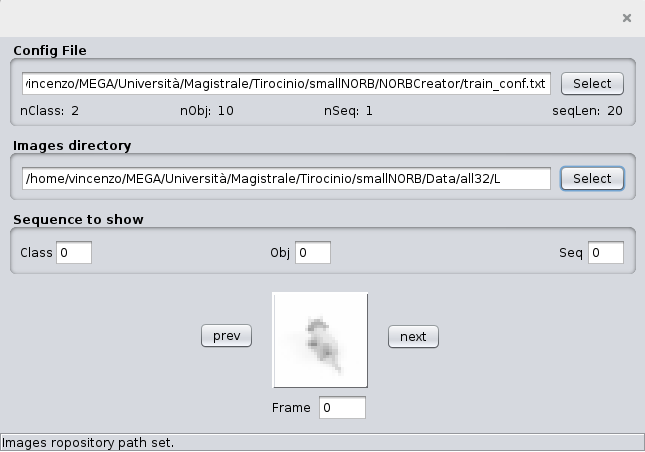
\includegraphics[width=\textwidth]{seqBrowser}
    \caption{Interfaccia dell'esploratore di sequenze}
\end{figure}

\section{NorbKNN.java}
\emph{NorbConverter.java} è una prima bozza di classificatore di base KNN. Esso utilizza la libreria \emph{weka} e per ogni sequenza crea un unico vettore di feature che giustappone le intensità dei pixel per ciascuna immagine.

\section{NorbCreator.java}
\emph{NorbCreator.java} si preoccupa di offrire un' interfaccia testuale per l'automatizazzione di tutte le funzionalità offerte.
Mediante la somministrazione da parte dell'utente di un unico file di configurazione completo di tutte le informazioni, infatti, è possibile passare direttamente alla visualizzazione delle sequenze create.

\subsection{Il formato del file di configurazione}
Il formato del file di configurazione è autoesplicativo e rappresenta l'unione di tutte le informazioni necessarie per svolgere la totalità delle operazioni descritte precedentemente.
Si consideri la Fig. \ref{img:configfile} come esempio.

\begin{figure}[H]
\label{img:configfile}
\centering
\begin{BVerbatim}
#########################
#      CONFIG FILE      #
#########################

#########################
#   CONVERSION PARAMS   #
#########################
matlabFile: ../Data/Matlab/smallnorb-5x46789x9x18x6x2x96x96-training-
destDir: ../Data/all32
convert(yes/no): no
inputWidth: 96
inputHeight: 96
scaleFactor: 3
#########################

#########################
#     COMMON PARAMS     #
#########################
imagesRepo: ../Data/all32/L
nClass: 2
nObjxClass: 10
elevationProb: 0.55
azimuthProb: 0.35
lightingProb: 0.1
flipProb: 0.05
seqLen: 40
#########################

#########################
#     TRAIN PARAMS      #
#########################
fileName: train_conf.txt
nSeqxObj: 1
seed: 1
#########################

#########################
#      TEST PARAMS      #
#########################
fileName: test_conf.txt
nSeqxObj: 1
seed: 2
minDistance: 0
#########################

#########################
#      END CONFIG       #
#########################

\end{BVerbatim}
\caption{Un esempio completo di file di configurazione.}
\end{figure}

\section{norbCreator.jar}
\emph{NorbCreator.jar} è un jar eseguibile contenente tutte le classi descritte precedentemente e le librerie indispensabili all'esecuzione.  Esso, quando invocato, esegue il main della classe di interfaccia \emph{NorbCreator.java} passandole gli opportuni parametri inseriti da line di comando. 
In particolare è possibile eseguire il jar secondo le seguenti modalità:

\begin{lstlisting}
1) java -jar norbCreator.jar configFileName
2) java -jar norbCreator.jar --convert configFileName
3) java -jar norbCreator.jar --sampleTrain configFileName
4) java -jar norbCreator.jar --sampleTest configFileName
5) java -jar norbCreator.jar --seqExplorer configFileName
\end{lstlisting}

Passando semplicemente il nome del file di configurazione tutte le sezioni vengono considerate e le conseguenti operazioni eseguite. Quindi, senza modificare alcuna linea di codice, è possibile tarare direttamente i paramentri nel file di configurazione, lanciare il programma e visualizzare le sequenze create non appena il browser farà la sua comparsa sullo schermo. 
Utilizzando invece gli opportuni flag solo le corrispondenti operazioni vengono svolte in maniera esclusiva.

%\begin{align} 
%\begin{split}
%(x+y)^3 	&= (x+y)^2(x+y)\\
%&=(x^2+2xy+y^2)(x+y)\\
%&=(x^3+2x^2y+xy^2) + (x^2y+2xy^2+y^3)\\
%&=x^3+3x^2y+3xy^2+y^3
%\end{split}					
%\end{align}

%Phasellus viverra nulla ut metus varius laoreet. Quisque rutrum. Aenean imperdiet. Etiam ultricies nisi vel augue. Curabitur ullamcorper ultricies

%------------------------------------------------

%\subsection{Heading on level 2 (subsection)}
%
%Lorem ipsum dolor sit amet, consectetuer adipiscing elit. 
%\begin{align}
%A = 
%\begin{bmatrix}
%A_{11} & A_{21} \\
%A_{21} & A_{22}
%\end{bmatrix}
%\end{align}
%Aenean commodo ligula eget dolor. Aenean massa. Cum sociis natoque penatibus et magnis dis parturient montes, nascetur ridiculus mus. Donec quam felis, ultricies nec, pellentesque eu, pretium quis, sem.
%
%%------------------------------------------------
%
%\subsubsection{Heading on level 3 (subsubsection)}
%
%\lipsum[3] % Dummy text
%
%\paragraph{Heading on level 4 (paragraph)}
%
%\lipsum[6] % Dummy text
%
%%----------------------------------------------------------------------------------------
%%	PROBLEM 2
%%----------------------------------------------------------------------------------------
%
%\section{Lists}
%
%%------------------------------------------------
%
%\subsection{Example of list (3*itemize)}
%\begin{itemize}
%	\item First item in a list 
%		\begin{itemize}
%		\item First item in a list 
%			\begin{itemize}
%			\item First item in a list 
%			\item Second item in a list 
%			\end{itemize}
%		\item Second item in a list 
%		\end{itemize}
%	\item Second item in a list 
%\end{itemize}
%
%%------------------------------------------------
%
%\subsection{Example of list (enumerate)}
%\begin{enumerate}
%\item First item in a list 
%\item Second item in a list 
%\item Third item in a list
%\end{enumerate}
%
%%----------------------------------------------------------------------------------------
%
\end{document}